\section{Признаки сходимости положительных рядов}

Пусть, $\baserow{a_n} = a_1 + a_2 + \dots + a_n + \dots = S$ --- сходящийся ряд, тогда
\[
    \text{частная сумма ряда }S_n = a_1 + a_2 + \dots + a_n \rightarrow S (n \rightarrow +\infty)
\]

И, если $\sum\limits_{n = 1}^{+\infty} |a_n|$ --- сходящийся ряд, то $\baserow{a_n}$ --- тоже сходится, причём абсолютно (абсолютная сходимость --- более ёмкое понятие)

\begin{Def}
	Числовой ряд $\baserow{a_n}$
	$\Leftrightarrow \forall n \in \bb{N} \: a_n \geq 0$
\end{Def}

\begin{Th}
	Пусть $\sum\limits_{n = 1}^{+\infty}a_n$ --- положительный ряд, частичные суммы $S_n$ которого ограничены сверху. Тогда ряд $\baserow{a_n} = S$ сходится и его сумма равна $S = \underset{n \geq 1}{sup}(S_n))$
\end{Th}
\begin{Proof}
	$\forall n \geq 1 \: S_{n+1} = S_n + a_n \geq S_n(\text{ряд положительный} \Rightarrow \\
	\Rightarrow a_{n+1} \geq 0) \Rightarrow \text{Послеовательность} \{S_n\}\nearrow.$ \\
	Тогда $\exists \lim\limits_{n \to +\infty} (S_n) \Leftrightarrow \text{последовательность } \{S_n\}$ ограничена сверху и её предел равен $S = \underset{n \geq 1}{sup}(S_n)$
\end{Proof}

 Короче, если из бесконечного множества частных сумм ряда ни одна не превышает какого-то числа, то ряд точно сходится. Причём схоится к большей из этого бесконечного числа сумм.

\begin{Th}[Признак сравнения сходимости рядов]
	Пусть $\baserow{a_n}$ и $\baserow{b_n}$ --- два ряда. При этом:
	\begin{enumerate}
		\item $\forall n \geq 1 \: a_n \geq 0$ (ряд положительный)
		\item $\exists n_0 \in \bb{N} \forall b \geq n_0 \: |b_n| \leq a_n$
		\item Ряд $\baserow{a_n} = S$ сходится
	\end{enumerate}
	Тогда $\baserow{b_n}$ сходится
\end{Th}

\begin{Proof}
     Ряд $\baserow{a_n}$ сходится $\Rightarrow$ [по критерию Коши] $\Rightarrow\\
	\Rightarrow $ \mbox{$\forall \varepsilon > 0 \: \exists N \geq n_0 \: \forall p \in \bb{N} \: \forall n \geq N \: |a_{n+1} + \dots + a_{n+p}| < \varepsilon$} $\Rightarrow\\
	\Rightarrow |b_{n+1} + \dots + b_{n+p}| \leq |b_{n+1}| + \dots + |b_{n+p}| \leq a_{n+1} + \dots + a_{n+p} = $[т.к. $a_n \geq 0$] $ = |a_{n+1} + \dots a_{n+p}| < \varepsilon$\\
	Т.е. $|b_{n+1} + \dots + b_{n+p}| < \varepsilon \Rightarrow$ [по критерию Коши] $\Rightarrow $ $\baserow{b_n}$ сходится.
\end{Proof}

\begin{Seq}
	$\forall n \geq n_0 \: 0 \leq b_n \leq a_n $ Если ряд $\baserow{b_n}$ расходится, то и $\baserow{a_n}$ тоже расходится
\end{Seq}

\begin{Proof}
	От противного:\\
	Если бы $\baserow{a_n}$ сходился, то по теореме 2 $\baserow{b_n}$ --- сходился бы $\Rightarrow$ противоречие
\end{Proof}

\begin{Th}[Признак сравнения рядов в предельной форме]
	Пусть $\forall n \geq 1 \: a_n \geq 0, b_n \geq 0$ и $\exists \lim\limits_{n \to +\infty}\frac{a_n}{b_n} = c \neq 0 \text{, т.е. } c > 0$\\
	Тогда ряд $\baserow{a_n}$ сходится $\Leftrightarrow$ ряд $\baserow{b_n}$ сходится
\end{Th}

\begin{Proof}
	$\Rightarrow$ $\baserow{a_n}$ сходится, $\lim\limits_{n \to +\infty} \frac{a_n}{b_n} = c \Rightarrow$\\
	Пусть $\varepsilon = \frac{c}{2} (\varepsilon > 0) \Rightarrow \exists n_0 \in \bb{N} \: \forall n \geq n_0 \: |\frac{a_n}{b_n} - c| < \frac{c}{2} \Rightarrow \frac{c}{2} < \frac{a_n}{b_n} < \frac{3c}{2} \Rightarrow\\
	\Rightarrow \forall n \geq n_0 \: 0 < b_n < \frac{2}{c}a_n$\\
	Ряд $\baserow{a_n}$ сходится $\Rightarrow$ [по теореме 2] $\Rightarrow$ $\baserow{b_n}$ сходится.\\
	$\Leftarrow$\\
	Ряд $\baserow{b_n}$ сходится $\Rightarrow \forall n \geq n_0 \: a_n < \frac{3}{2}cb_n \Rightarrow$ [по теореме 2] $\Rightarrow\\
	\Rightarrow$ $\baserow{a_n}$ сходится 
\end{Proof}

Аналогичная штука работает для расходящихся рядов:\\
Если предел отношения элементов ряда на бесконечности равен ненулевой константе и один из рядов расходящийся, то и второй тоже обязательно расходится

\begin{Example}
	$\;$ \newline
	\begin{enumerate}
		\item ряд $\baserow{\ln(1+\frac{1}{n})}$ расходится $(1)$ \\
			$\ln(1+t) \sim t (t \to 0) \Rightarrow [t=\frac{1}{n}] \Rightarrow \ln(1+\frac{1}{n}) \sim \frac{1}{n} (n \to +\infty) \Rightarrow\\
			\Rightarrow \lim\limits_{n \to +\infty} \frac{\ln(1+\frac{1}{n})}{\frac{1}{n}} = 1 \neq 0$ \\
			Теперь, учитывая, что у нас есть ненулевой предел отношения элементов двух рядов, один из которых расходящийся, можно говорить, что расходится и второй, т.е. ряд $\baserow{\frac{1}{n}}$ расходится
		\item ряд $\baserow{\frac{1}{n(n+1)}} = 1$ сходится. $(S_n = 1 - \frac{1}{n+1}) \Rightarrow$ ряд $\baserow{\frac{1}{n^2}}$ сходится, т.к. $\lim\limits_{n \to +\infty}\frac{\frac{1}{n(n+1)}}{\frac{1}{n^2}} = 1$
	\end{enumerate}
\end{Example}

\begin{Th}[Признак Даламбера]
	Пусть $\forall n \geq 1 \: a_n > 0$ и:
	\begin{enumerate}
		\item $\exists q < 1 \: \forall n \geq n_0 \; \frac{a_{n+1}}{a_n} \leq q \leq 1$. Тогда ряд $\baserow{a_n}$ сходится
		\item $\forall n \geq n_0 \; \frac{a_{n+1}}{a_n} \geq 1 \Rightarrow $ ряд $\baserow{a_n}$ расходится
	\end{enumerate}
\end{Th}

\begin{Proof}
	\begin{enumerate}
		\item $\frac{a_{n+1}}{a_n} \leq q < 1 (\forall n \geq n_0)$\\
		$a_n \leq a_{n-1}q \leq a_{n-2}q^2 \leq \dots \leq a_{n_0}q^{n-n_0}$\\
		$\sum\limits_{n=n_0}^{+\infty}a_{n_0}q^{n-n_0} = a_{n_0}\sum\limits_{k = 0}^{+\infty}q^k = \frac{a_{n_0}}{1-q}$ сходится, т.к. $0 < q < 1 \Rightarrow \\
		\Rightarrow [\text{по теореме 2}] \Rightarrow$ $\baserow{a_n}$ сходится
		\item $\forall n \geq n_0 \; \frac{a_{n+1}}{a_n} \geq 1 \Rightarrow a_n \geq a_{n-1} \geq \dots \geq a_{n_0} > 0 \Rightarrow a_n \geq a_{n_0} > 0\\
		n \to +\infty $, если бы $a_n \to 0$ (условие сходимости ряда), тогда по принципу сжатой переменной $a_{n_0} = 0$, но это не так $\Rightarrow$ противоречие $\Rightarrow a_n \nrightarrow 0 (n \to +\infty)$ и ряд расходится
	\end{enumerate}
\end{Proof}

\begin{Th} [Признак Даламбера в предельной форме]
	Пусть $\forall n \geq 1 \: a_n > 0$ и $\exists \lim\limits_{n \to +\infty}\frac{a_{n+1}}{a_n} = q$, тогда:
	\begin{enumerate}
		\item $q < 1 \Rightarrow$  $\baserow{a_n}$ сходится
		\item $q > 1 \Rightarrow$  $\baserow{a_n}$ расходится
		\item $q = 1 \Rightarrow$  $\baserow{a_n}$ может сходиться или расходиться
	\end{enumerate}
\end{Th}

\begin{Proof}
	$\:$ \\
	\begin{enumerate}
		\item $\lim\limits_{n \to +\infty}\frac{a_{n+1}}{a_n} = q, q < 1$\\
		$q<1 \Rightarrow \varepsilon = \frac{1-q}{2} > 0 \exists n_0 \in \bb{N} \: \forall n \geq n_0 \; |\frac{a_{n+1}}{a_n}-q| < \frac{1-q}{2} \Rightarrow\\
		\Rightarrow q-\frac{1-q}{2} < \frac{a_{n+1}}{a_n} < q+\frac{1-q}{2} = \frac{q+1}{2} = q^{\ast} < \frac{2}{2} = 1 \Rightarrow \\
		\Rightarrow \forall n \geq n_0 \: \frac{a_{n+1}}{a_n} < q^{\ast} < 1 \Rightarrow [\text{по теореме 4}] \Rightarrow$ $\baserow{a_n}$ сходится
		\item $\lim\limits_{n \to +\infty}\frac{a_{n+1}}{a_n} = q > 1 \Rightarrow \varepsilon = \frac{q-1}{2} > 0$ \\
		$\exists n_0 \in \bb{N} \: \forall n \geq n_0 \: |\frac{a_{n+1}}{a_n} - q| < \frac{q-1}{2} \Rightarrow q-\frac{q-1}{2} < \frac{a_{n+1}}{a_n} < q+\frac{q-1}{2}$\\
		$1 = \frac{1 + 1}{2} < q^{\ast} = \frac{q+1}{2} < \frac{a_{n+1}}{a_n} > q^{\ast} > 1 \Rightarrow [\text{по теореме 4}] \Rightarrow$ $\baserow{a_n}$ расходится
		\item $q=1: \lim\limits_{n \to +\infty}\frac{a_{n+1}}{a_n} = 1$\\
		Тут достаточно привести примеры сходящегося и расходящегося ряда для $q = 1$:
		\begin{itemize}
			\item $\baserow{\frac{1}{n}}$ расходится, $\frac{a_{n+1}}{a_n} = \frac{n}{n+1} \to 1 (n \to +\infty)$
			\item $\baserow{\frac{1}{n^2}}$ сходится, $\frac{a_{n+1}}{a_n} = \frac{n^2}{(n+1)^2} \to 1 (n \to +\infty)$
		\end{itemize}
	Итого точно сказать нельзя
	\end{enumerate}
\end{Proof}

\begin{Th}[Радикальный метод Коши]
	Пусть $\forall n \geq 1 \; a_n > 0 \; \text{и} \\ 
	\exists \lim\limits_{n \to +\infty}\sqrt[n]{a_n} = l, l \in \bb{R}.$ Тогда, если:
	\begin{enumerate}
		\item $l < 1 \Rightarrow$ $\baserow{a_n}$ сходится
		\item $l > 1 \Rightarrow$ $\baserow{a_n}$ расходится
		\item $l = 1 \Rightarrow$ $\baserow{a_n}$ не определено. Может сходиться или расходиться
	\end{enumerate}
\end{Th}

\begin{Proof}
	$\:$ \\
	\begin{enumerate}
		\item $0 \geq l < 1 (\text{т.к. l это корень})$\\
		$\varepsilon = \frac{1-l}{2} \; \exists n_0 \in \bb{N} \: \forall n \geq n_0 \; |\sqrt[n]{a_n} - l| < \frac{1-l}{2} \Rightarrow \\
		\Rightarrow \sqrt[n]{a_n} < \frac{l+1}{2} = l^{\ast} < 1 \Rightarrow a_n < (l^{\ast})^n (n \geq n_0), l^{\ast} \in [0;1]$\\
		ряд $\sum\limits_{n = n_0}^{+\infty}(l^{\ast})^n =\\
		= [\text{Как сумма геом. прогрессии со знаменателем меньшим единицы}] =\\
		= \frac{(l^{\ast})^{n_0}}{1 - l^{\ast}}$ сходится $\Rightarrow$ $\baserow{(l^{\ast})^n}$ сходится $\Rightarrow$ [по теореме 3] $\Rightarrow$ тоже сходится
		\item $l > 1 \Rightarrow \varepsilon = \frac{l-1}{2} \; \exists n_0 \in \bb{N} \: \forall n \geq n_0 \; |\sqrt[n]{a_n} - l| < \frac{l-1}{2} \Rightarrow \\
		\Rightarrow 1 < l^{ast} = \frac{l+1}{2} = l - \frac{l-1}{2} < \sqrt[n]{a_n} (n \geq n_0) \Rightarrow \\
		\Rightarrow \forall n \geq n_0 a_n > 1 \Rightarrow a_n \nrightarrow 0 (n \to +\infty) \Rightarrow$ ряд $\baserow{a_n}$ расходится
		\item Тут тоже достаточно только привести примеры:
		\begin{itemize}
			\item $\baserow{1}$ $a_n = 1, \sqrt[n]{a_n} = 1, \sqrt[n]{a_n} \to 1 (n \to +\infty) \Rightarrow l=1$, а ряд расходится
			\item $\baserow{\frac{1}{n^2}}$, $\sqrt[n]{a_n} = (\frac{1}{n^2})^{\frac{1}{n}} = e^{-2\frac{\ln n}{n}} \to 1 (n \to +\infty) \\
			(\text{т.к. логарифм возрастает медленее 1й степени и степень е стремится к 0}) \Rightarrow l = 1$, а ряд расходится
		\end{itemize}
	\end{enumerate}
\end{Proof}

\begin{Th}[Интегральный признак Коши]
	Пусть функция $f(x)$ удовлетворяет условиям:
	\begin{enumerate}
		\item $f(x) \in C_{[1;+\infty)}$
		\item $f(x) \searrow$ на $[1;+\infty)$
		\item $\forall x \in [1; + \infty) \; f(x) > 0$
	\end{enumerate}
	Тогда ряд $\baserow{f(n)}$ сходится $\Leftrightarrow$ несобственный интеграл $\int\limits_{1}^{+\infty}f(x)\,dx$ сходится
\end{Th}

\begin{Proof}
	$\:$ \\
	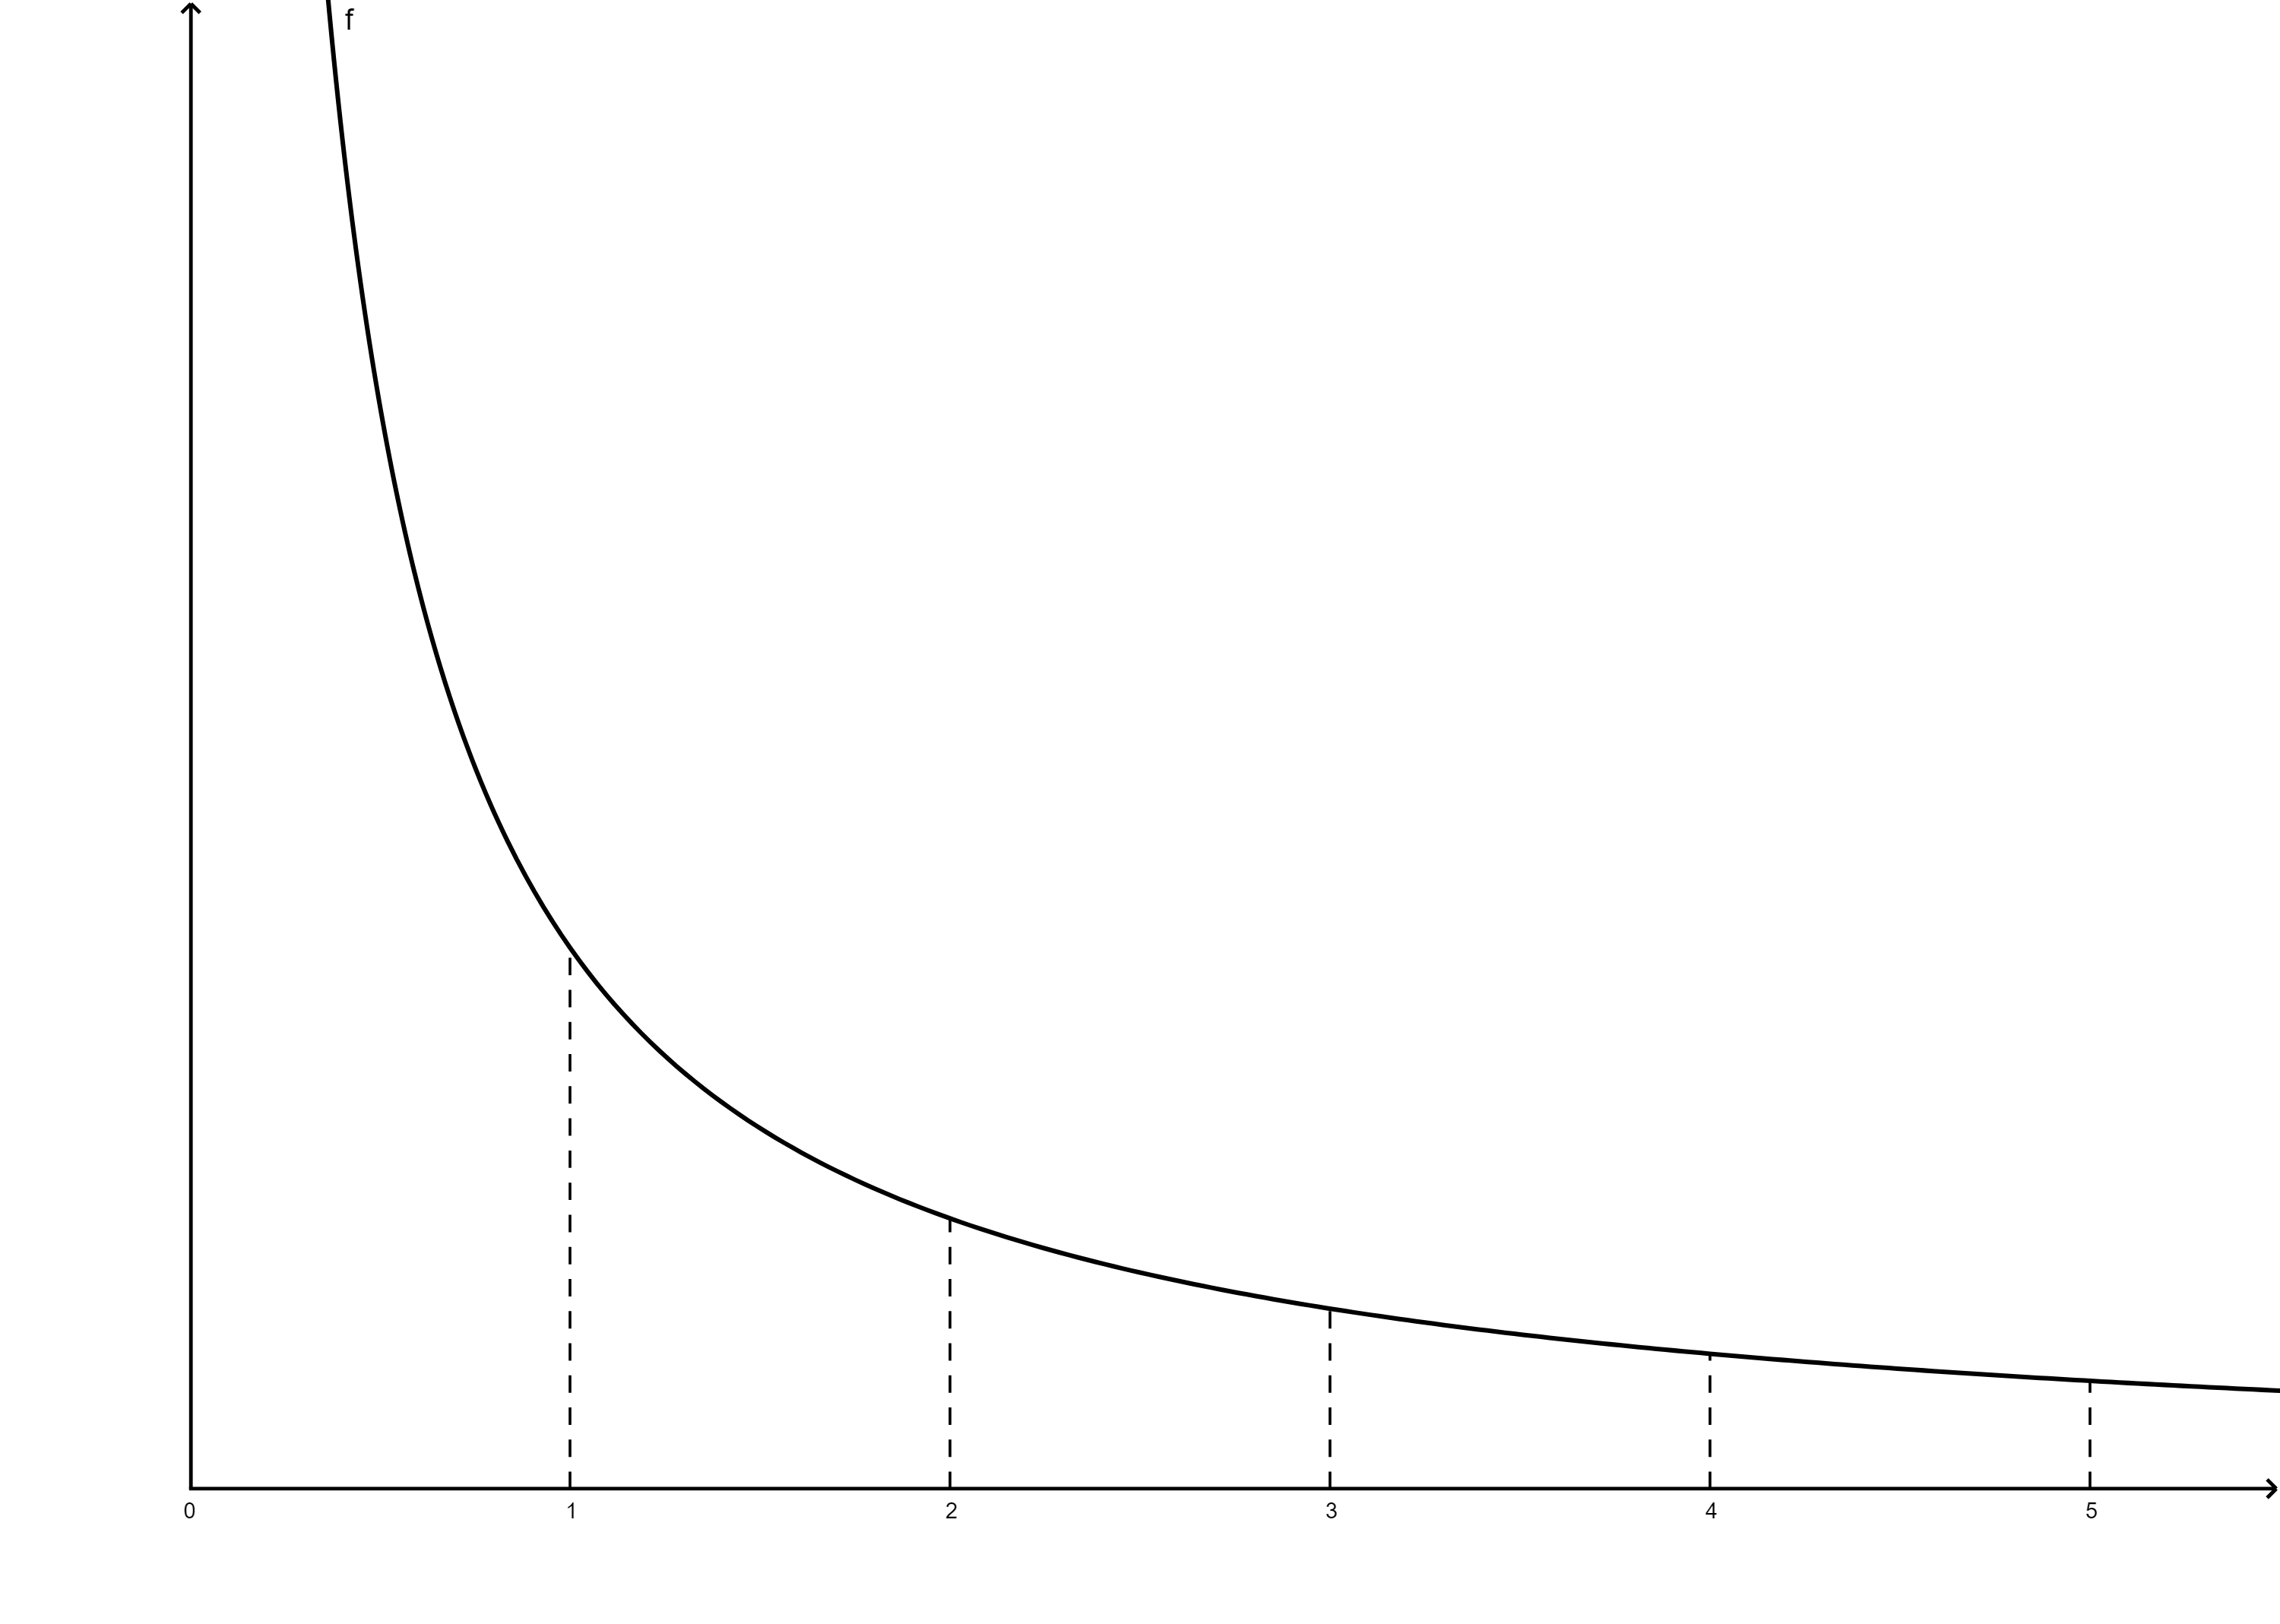
\includegraphics[width=0.5\linewidth]{pictures/3_2_1.png}\\
	$x \in [k; k+1], f(k+1) < f(x) < f(k) (k=1,2,\dots) \Rightarrow \\
	\Rightarrow f(k+1) \leq \int\limits_{k}^{k+1}f(x)\,dx \leq f(k) \Rightarrow \\
	\Rightarrow \sum\limits_{k=1}^{n}f(k+1) \leq \int\limits_{1}^{n+1}f(x)\,dx \leq \sum\limits_{k=1}^{n}f(k) = S_n, S_{n+1} - f(1) \leq \int\limits_{1}^{n+1}f(x)\,dx \leq S_n$\\
	$\Rightarrow$: \\
	$\baserow{f(n)}$ сходится $\Rightarrow$ [по теореме 1] $\Rightarrow S_n \leq S$\\
	$\forall t \in \bb{R} \; t > 1 \; \exists n \in \bb{N} t<n+1$ (аксиома Архимеда)\\
	$F(t) = \int\limits_{1}^{t}f(x)\,dx = \int\limits_{1}^{n+1}f(x)\,dx \leq S_n \ leq S$\\
	$F(t) \nearrow$ т.к. $F'=f(x) \Rightarrow \exists \lim\limits_{t \to +\infty} = F \leq S \Rightarrow \int\limits_{1}^{+\infty}f(x)\,dx$ сходится\\
	$\Leftarrow$:\\
	$\int\limits_{1}^{+\infty}f(x)\,dx = F$ сходится $\Rightarrow S_n \leq f(1) + \int\limits_{1}^{n+1}f(x)\,dx \leq f(1) + F \Rightarrow \\
	\Rightarrow [\text{по теореме 1}] \Rightarrow$ $\baserow{f(n)}$ сходится
\end{Proof}